
%%%%%
%%%%% DO NOT EDIT THIS FILE
%%%%%



\documentclass[12pt,a4paper,fleqn]{report}

%%% packages for mathematical typesetting
\usepackage{amsmath}
\usepackage{amssymb}
\usepackage{times}
\usepackage{bm}
%\usepackage{mathtools}
%\usepackage{nicefrac}
%\usepackage{latexsym}

%%% packages for including figures and subfigures
\usepackage{graphicx}
\usepackage[font=footnotesize,labelformat=empty]{subfig}

%%% package for nicer table layout
\usepackage{booktabs}
\usepackage{colortbl}

%%% package for color mangement
\usepackage[svgnames]{xcolor}

%%% package for page headings and footers
\usepackage{fancyhdr}

%%% package for hyperlinks
\usepackage{hyperref}
\hypersetup{%
  colorlinks=true,
  urlcolor=DarkGreen,
  citecolor=green,
  bookmarks=false}


\usepackage[noend]{algpseudocode}
\algrenewcommand\algorithmicdo{}
\algrenewcommand\algorithmicthen{}
\algrenewcommand{\algorithmiccomment}[1]{// #1}
\makeatletter
\newcommand{\StatexIndent}[1][3]{%
  \setlength\@tempdima{\algorithmicindent}%
  \Statex\hskip\dimexpr#1\@tempdima\relax}
\makeatother


\usepackage{fancyvrb} 
\usepackage{listings}
% Python style / environment for highlighting in "figures"
\lstdefinestyle{pythonstyle}{%
  language=Python,
  tabsize=4,
  backgroundcolor=\color{Gray!10},
  basicstyle=\ttfamily\scriptsize,
  stringstyle=\color{ForestGreen},
  keywordstyle=\color{BlueViolet},
  commentstyle=\itshape\color{DarkRed!90},
  identifierstyle=,
  emphstyle=\color{Blue},
  frame=lines,	
  showstringspaces=false,
  morekeywords={range, len, self, lambda, from, import, as, False, True, enumerate, map, list, set, float, int, min, max, with}
  fancyvrb=true,
}
\lstnewenvironment{python}[1][]{\lstset{style=pythonstyle,#1}}{}





\graphicspath{{./Figures/}, {./Images/}}



%%% text highlighting
\newcommand{\keyword}[1]{\emph{\texttt{\color{blue}#1}}}
\newcommand{\alert}[1]{\emph{\texttt{\color{red}#1}}}


%%% sets
\newcommand{\set}[1]{#1}

%%% vectors, matrices, and tensors
\renewcommand{\vec}[1]{\bm{#1}}
\newcommand{\mat}[1]{\bm{#1}}
\newcommand{\ten}[1]{\bm{\mathcal{#1}}}

%%% trace, rank, and diagonal
\newcommand{\tr}[1]{\operatorname{tr} \bigl [ #1 \bigr ]}
\newcommand{\TR}[1]{\operatorname{tr} \Bigl [ #1 \Bigr ]}
\newcommand{\rk}[1]{\operatorname{rk} \bigl [ #1 \bigr ]}
\newcommand{\RK}[1]{\operatorname{rk} \Bigl [ #1 \Bigr ]}
\newcommand{\diag}[1]{\operatorname{diag} \bigl [ #1 \bigr ]}
\newcommand{\DIAG}[1]{\operatorname{diag} \Bigl [ #1 \Bigr ]}

%%% inverse and transpose
\newcommand{\inv}[1]{#1^{-1}}
\newcommand{\trn}[1]{#1^\intercal}
\newcommand{\invtrn}[1]{#1^{-\intercal}}

%%% outer product
\newcommand{\opt}[2]{#1 \trn{#2}}

%%% inner products
\newcommand{\ipt}[2]{\trn{#1} #2}
\newcommand{\iptb}[2]{\left( \ipt{#1}{#2} \right)}
\newcommand{\ip}[2]{\langle #1, #2 \rangle}
\newcommand{\Ip}[2]{\bigl \langle #1, #2 \bigr \rangle}
\newcommand{\ipa}[2]{\langle #1, #2 \rangle}
\newcommand{\Ipa}[2]{\bigl \langle #1, #2 \bigr \rangle}
\newcommand{\dsq}[2]{\bigl \lVert #1 - #2 \bigr \rVert^2}
\newcommand{\nrm}[1]{\bigl \lVert #1 \bigr \rVert^2}
\newcommand{\sdsq}[2]{\lVert #1 - #2 \rVert^2}
\newcommand{\snrm}[1]{\lVert #1 \rVert^2}


\newcommand{\st}{\operatorname{s.\!t.}}
\newcommand{\amin}[1]{\operatorname*{argmin}_{#1}}
\newcommand{\amax}[1]{\operatorname*{argmax}_{#1}}

\newcommand{\submax}[1]{#1_{\text{max}}}

\newcommand{\ci}{\perp\!\!\!\perp}
\newcommand{\prob}[1]{p\bigl( #1 \bigr)}
\newcommand{\cprob}[2]{p\bigl( #1 \bigm| #2 \bigr)}

%%% horizontal and vertical dash
\newcommand{\hdash}{\operatorname{\,{}---{}\,}}
\renewcommand{\vdash}{\arrowvert}





\pagestyle{fancy}
\lhead{\emph{Pattern Recognition (2)}}
\rhead{\emph{Summer Term 2021}}
\cfoot{}

\frenchspacing

\setlength{\parskip}{1ex plus0.5ex minus0.5ex}

\setlength{\headheight}{15pt}

\def\thesection{\arabic{section}.}
\setlength{\parindent}{0pt}

\renewcommand{\familydefault}{\sfdefault}





\begin{document}

\subsection*{exercise 2}
\textbf{groups, complex numbers, and flows}
\vspace{1cm}

\subsection*{solutions due}
until \textbf{May 09, 2021} at \textbf{23:59} via \textbf{E-Mail}

\begin{tabular}{l l}
Fabrice: & s6fabeau[at]uni-bonn.de \\
Sebastian: & muellers[at]cs.uni-bonn.de
\end{tabular}

\vspace{1cm}

\vfill


\subsection*{students handing in this solution set}

\begin{tabular*}{\textwidth}{l@{\extracolsep{\fill}}lll}
  \toprule
  last name & first name & student ID & enrolled with \\
  \midrule
  \midrule
  Nikolskyy
  & Oleksander
  & TODO
  & TODO
  \\
  Schier
  & Marie
  & TODO
  & TODO
  \\
  Doll
  & Niclas
  & 3075509
  & Uni Bonn
  \\
  Safavi
  & Arash
  & TODO
  & TODO
  \\
  Wani
  & Mohamad Saalim
  & TODO
  & TODO
  \\
  Bonani
  & Mayara Everlim
  & TODO
  & TODO
  \\
  \bottomrule
\end{tabular*}
\newpage

%%%%%
%%%%% DO NOT EDIT THE FOLLOWING
%%%%%

\subsection*{general remarks}

As you know, your instructor is an avid  proponent of open science and education. Therefore, \textbf{MATLAB implementations will not be accepted} in this course.

The goal of this exercise is to get used to scientific Python. There are numerous resources on the web related to Python programming. Numpy and Scipy are well documented and Matplotlib, too, comes with numerous tutorials. Play with the code that is provided. Most of the above tasks are trivial to solve, just look around for ideas as to how it can be done.

Remember that you have to achieve at least 50\% of the points of the exercises to be eligible to the written exam at the end of the semester. Your grades (and credits) for this course will be decided based on the exam only, but --once again-- you have to succeed in the exercises to get there.
  
Your solutions have to be \emph{satisfactory} to count as a success. Your code and results will be checked and need to be convincing.

If your solutions meets the above requirements and you can demonstrate that they work in practice, it is a \emph{satisfactory} solution.

A \emph{very good} solution (one that is rewarded full points) requires additional efforts especially w.r.t. to readability of your code. If your code is neither commented nor well structured, your solution is not good! The same holds for your discussion of your results: these should be concise and convincing and demonstrate that you understood what the respective task  was all about. Striving for very good solutions should always be your goal!
 



\subsection*{practical advice}



The problem specifications you'll find below assume that you use python / numpy / scipy for your implementations. They also assume that you have imported the following
\begin{python}
import numpy as np
import numpy.linalg as la
import matplotlib.pyplot as plt
\end{python}


\subsection*{task 2.1 [5 points] \\[1ex] the dihedral group $D_3$}

\textbf{NOTE:} If you decide to give this task a try, then really try to solve it yourself! Those who do not like to- or cannot think for themselves may of course just go to wikipedia and look up the solution \ldots but what would you gain from that? 

The following are the six symmetries (three rotations and three reflections) of a unilateral triangle:

\begin{center}
\begin{tabular}{cc}
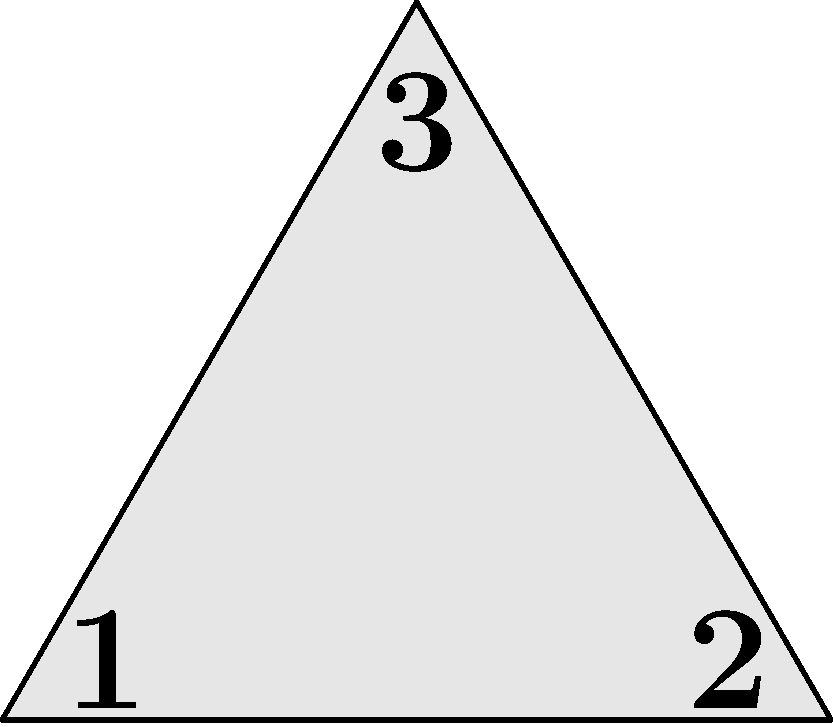
\includegraphics[width=0.1\textwidth]{triangle-I.pdf} \raisebox{2ex}{$\stackrel{I}{\rightarrow}$} 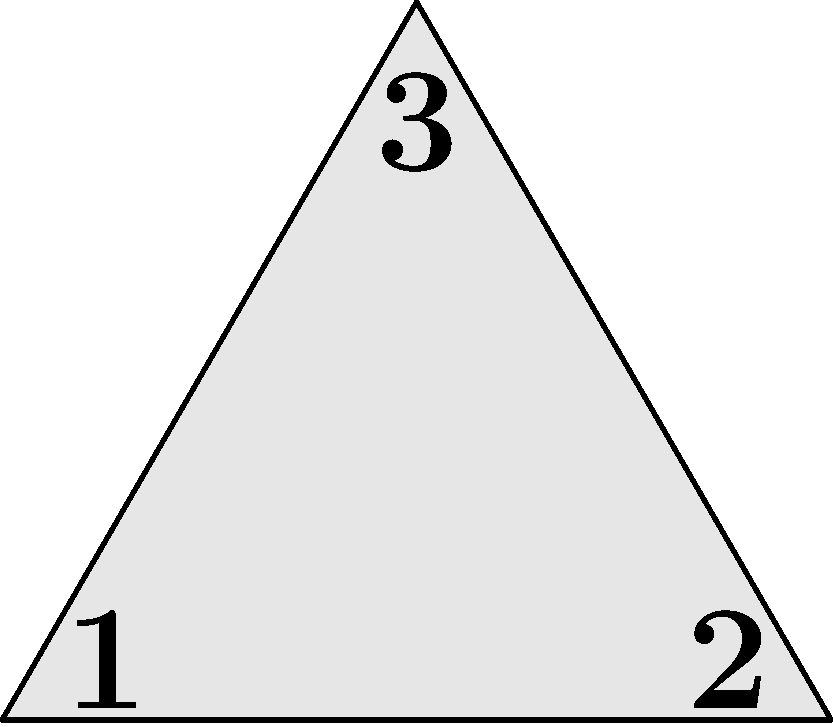
\includegraphics[width=0.1\textwidth]{triangle-I.pdf} \qquad
& \qquad 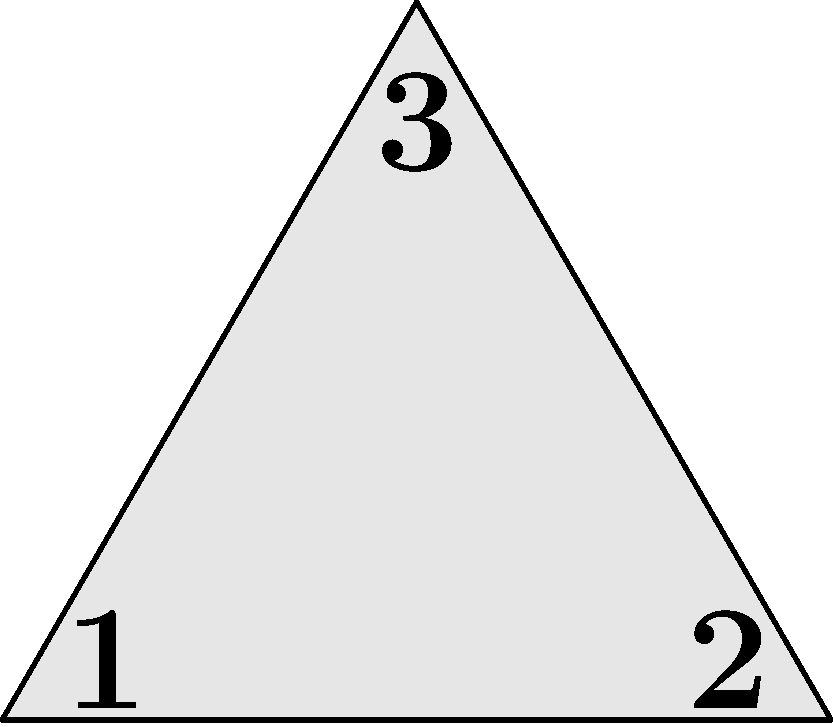
\includegraphics[width=0.1\textwidth]{triangle-I.pdf} \raisebox{2ex}{$\stackrel{F_1}{\rightarrow}$} 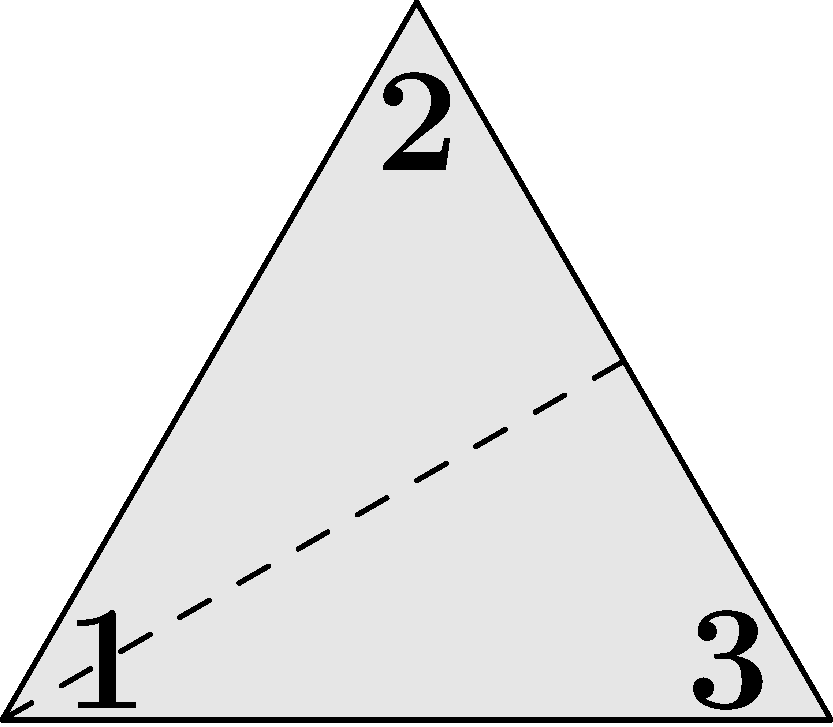
\includegraphics[width=0.1\textwidth]{triangle-F1.pdf} \\

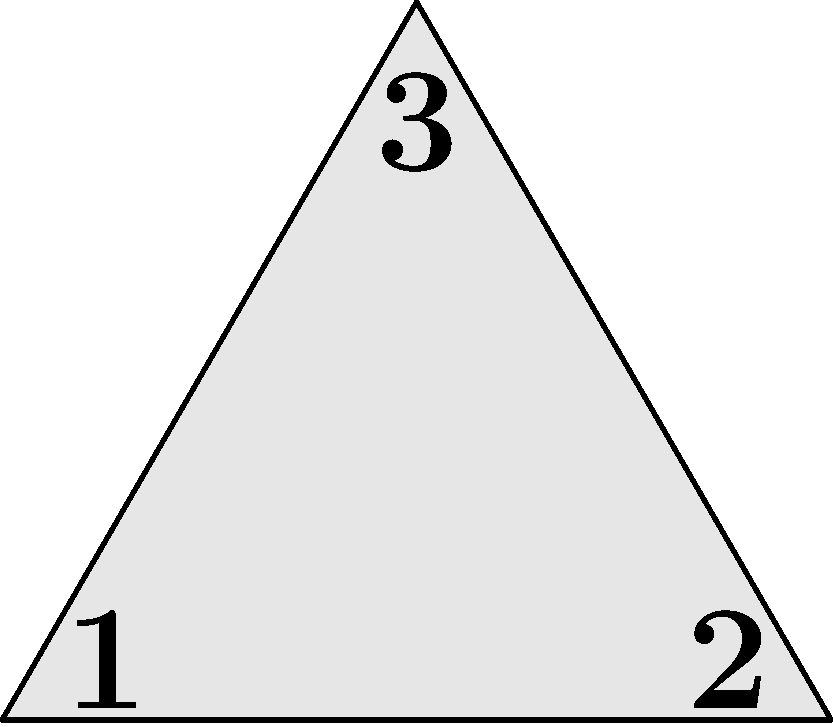
\includegraphics[width=0.1\textwidth]{triangle-I.pdf} \raisebox{2ex}{$\stackrel{R_1}{\rightarrow}$} 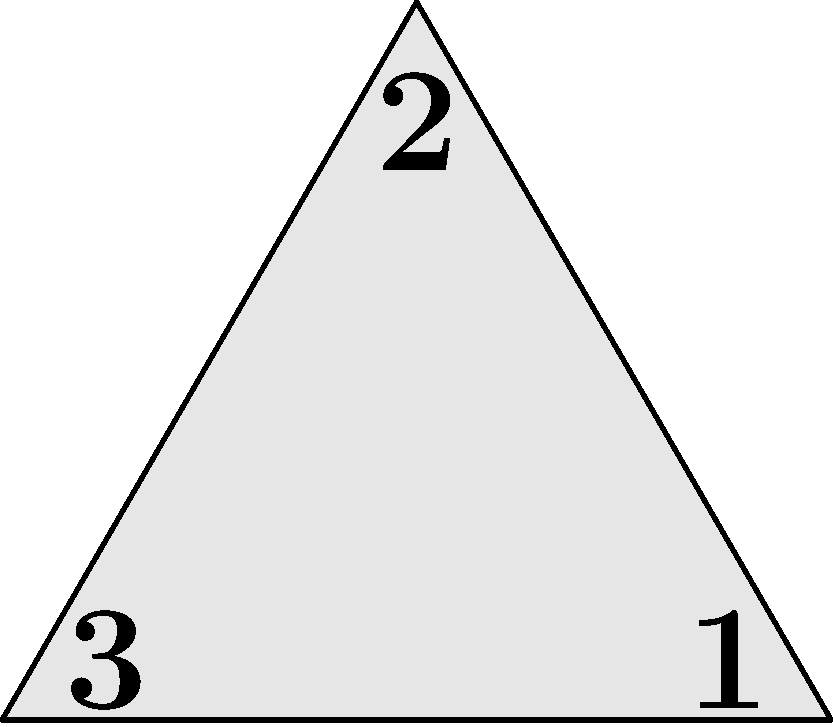
\includegraphics[width=0.1\textwidth]{triangle-R1.pdf} \qquad
& \qquad 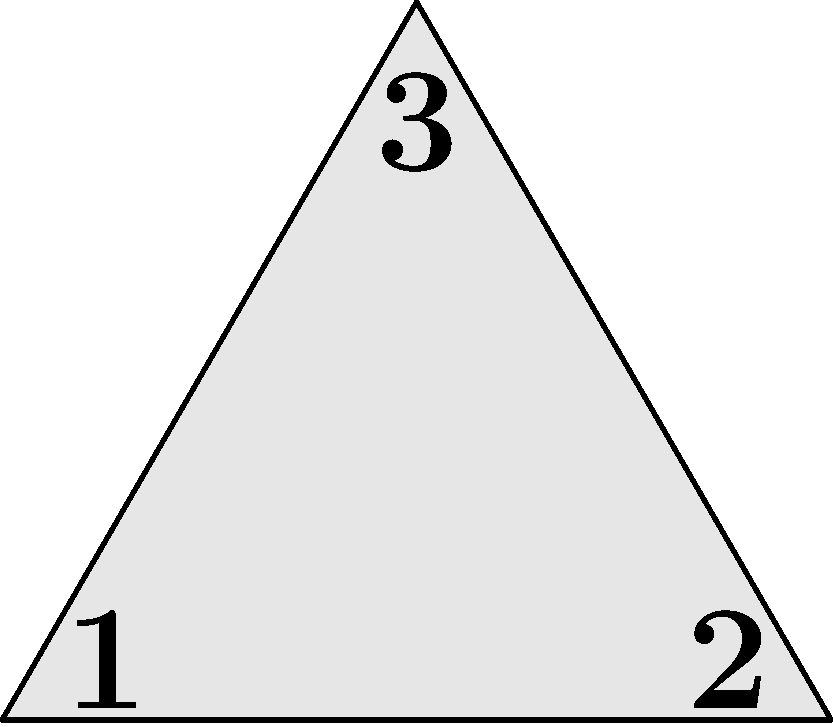
\includegraphics[width=0.1\textwidth]{triangle-I.pdf} \raisebox{2ex}{$\stackrel{F_2}{\rightarrow}$} 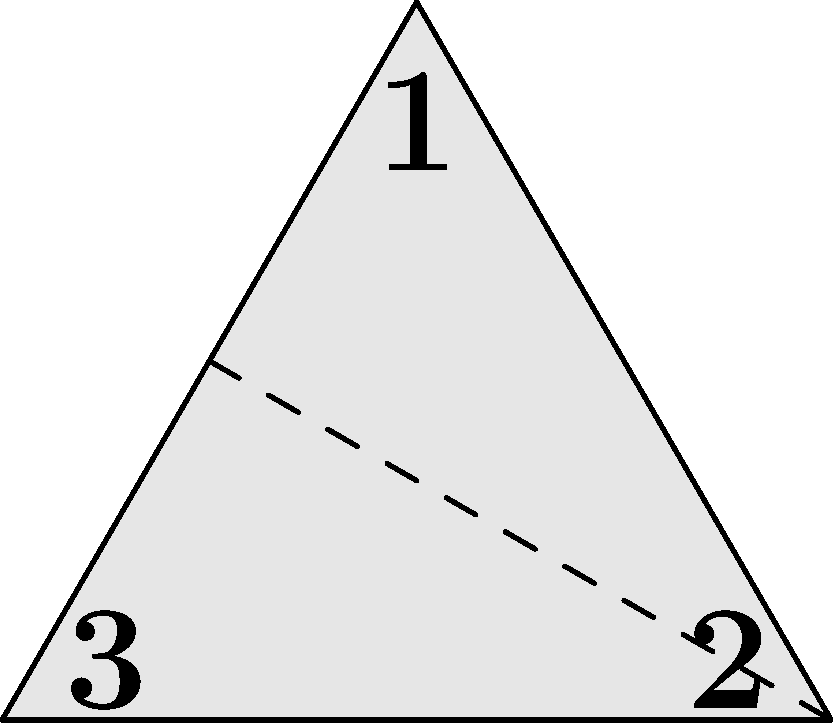
\includegraphics[width=0.1\textwidth]{triangle-F2.pdf} \\

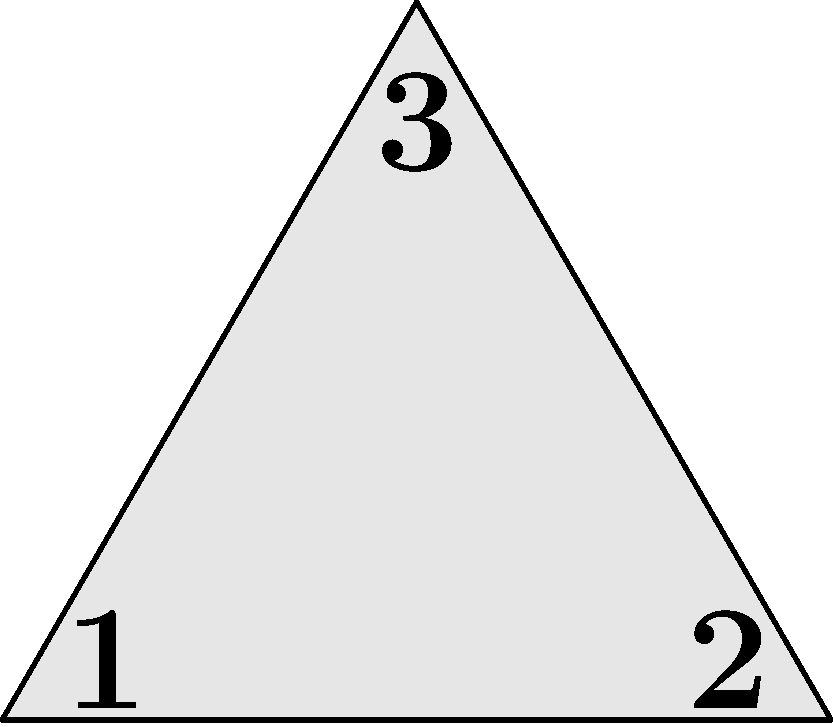
\includegraphics[width=0.1\textwidth]{triangle-I.pdf} \raisebox{2ex}{$\stackrel{R_2}{\rightarrow}$} 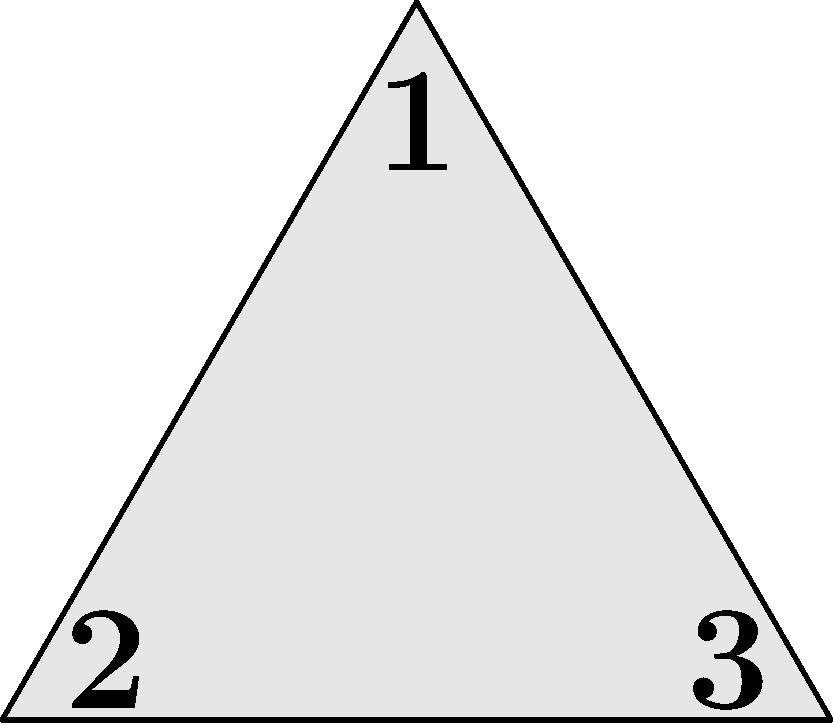
\includegraphics[width=0.1\textwidth]{triangle-R2.pdf} \qquad
& \qquad 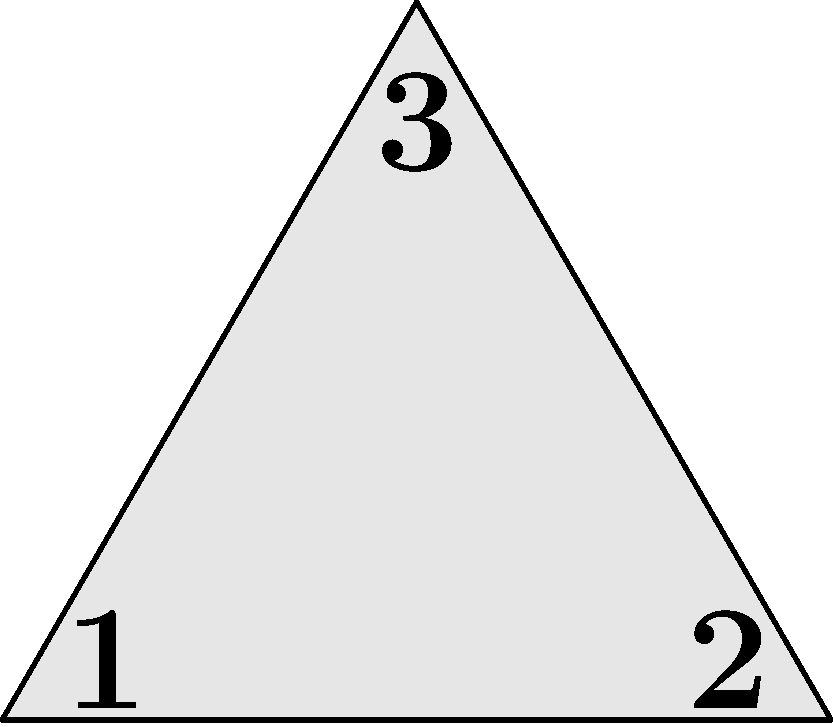
\includegraphics[width=0.1\textwidth]{triangle-I.pdf} \raisebox{2ex}{$\stackrel{F_3}{\rightarrow}$} 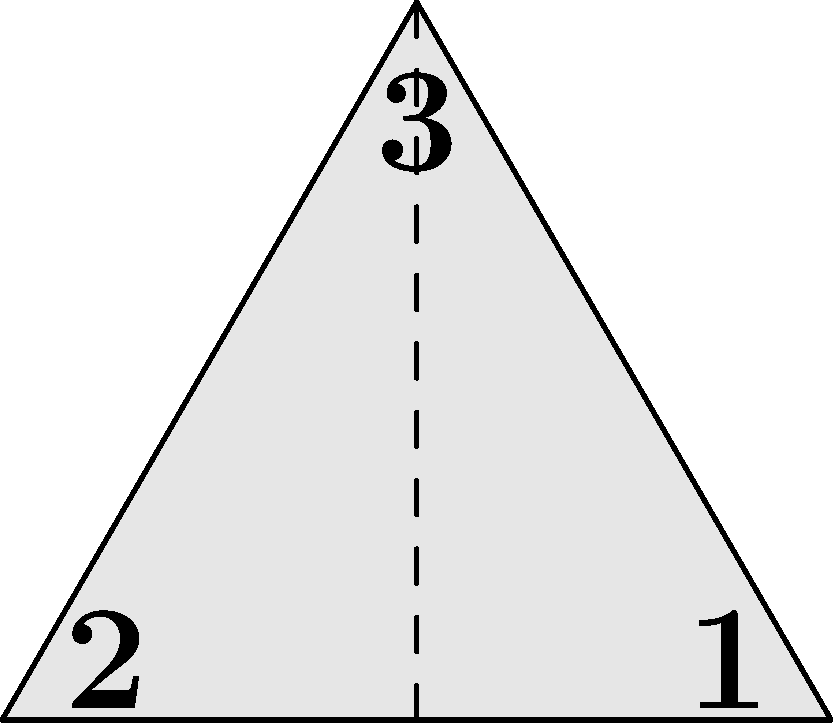
\includegraphics[width=0.1\textwidth]{triangle-F3.pdf}
\end{tabular}
\end{center}

Using the notation introduced in this figure, the dihedral group $D_3 = \bigl( G, \circ \bigr)$ consists of the following elements
\begin{align*}
G & = \bigl\{ I, R_1, R_2, F_1, F_2, F_3 \bigr\}
\intertext{and the group law}
\circ & \,:\, G \times G \rightarrow G
\end{align*}
is the composition, i.e. sequential execution, of any two operations in $G$. Given this information, complete the Cayley table for this group:
%%%%%
%%%%%
%%%%% complete the following table, i.e. replace the \ldots with the appropriate expression
%%%%%
%%%%%
\begin{center}
  \begin{tabular}{>{\columncolor[gray]{0.8}}cccccccc}
  \rowcolor[gray]{0.8} $\circ$ & $I$ & $R_1$ & $R_2$ & $F_1$ & $F_2$ & $F_3$ \\
  $I$   &  $I$  & $R_1$ & $R_2$ & $F_1$ & $F_2$ & $F_3$ \\
  $R_1$ & $R_1$ & $R_2$ &  $I$  & $F_2$ & $F_3$ & $F_1$ \\
  $R_2$ & $R_2$ &  $I$  & $R_1$ & $F_3$ & $F_1$ & $F_2$ \\
  $F_1$ & $F_1$ & $F_3$ & $F_2$ &  $I$  & $R_2$ & $R_1$ \\ 
  $F_2$ & $F_2$ & $F_1$ & $F_3$ & $R_1$ &  $I$  & $R_2$ \\
  $F_3$ & $F_3$ & $F_2$ & $F_1$ & $R_2$ & $R_1$ &  $I$   
  \end{tabular}
\end{center}
%%%%%
%%%%%
%%%%% complete the following table, i.e. replace the \ldots with the appropriate expression
%%%%%
%%%%%
\vspace{1ex}

Does your result ($\Leftrightarrow$ the structure of the completed table) suggest that $D_3$ is an Abelian group or not ?
\color{blue} \\[1ex]
%%%%%
%%%%%
%%%%% enter your discussion here
%%%%%
%%%%%
The Caylay table shows that the composition $\circ: G \times G \rightarrow G$ is not symmetric which implied that $D_3$ is not an Abelian group.
%%%%%
%%%%%
%%%%%
%%%%%
%%%%%
\color{black}


\subsection*{task 2.2 [5 points] \\[1ex] the quaternion group $Q_8$}

\textbf{NOTE:} If you decide to give this task a try, then once again really try to solve it yourself!

Recall that any complex number $z \in \mathbb{C}$ can be written as $z = a \cdot 1 + b \cdot i$ where $1, a, b \in \mathbb{R}$ and $i = \sqrt{-1}$. 

Also recall that complex numbers can be thought of as living in a 2D space called the complex plane.

In 1843, Hamilton famously extended the idea of complex numbers to 4D and introduced the \emph{quaternions} $q \in \mathbb{H}$ where
\begin{equation*}
q = a \cdot 1 + b \cdot i + c \cdot j + d \cdot k
\end{equation*}
Here, $a, b, c, d \in \mathbb{R}$ and the \emph{unit quaternions} $i, j, k$ are defined by their properties / multiplication rules
\begin{align*}
i^2 & = -1 & j^2 & = -1 & k^2 & = -1 & ijk & = -1 \\[1ex]
ij & = k & jk & = i & ki & = j \\
ji & = -k & kj & = -i & ik & = -j
\end{align*}

Given this information, complete the Cayley table for this group:
%%%%%
%%%%%
%%%%% complete the following table, i.e. replace the \ldots with the appropriate expression
%%%%%
%%%%%
\begin{center}
  \begin{tabular}{>{\columncolor[gray]{0.8}}ccccccccc}
  \rowcolor[gray]{0.8} $\cdot$ & $+1$ & $-1$ & $+i$ & $-i$ & $+j$ & $-j$ & $+k$ & $-k$ \\
  $+1$  & $+1$ & $-1$ & $+i$ & $-i$ & $+j$ & $-j$ & $+k$ & $-k$ \\
  $-1$  & $-1$ & $+1$ & $-i$ & $+i$ & $-j$ & $+j$ & $-k$ & $+k$ \\
  $+i$  & $+i$ & $-i$ & $-1$ & $+1$ & $+k$ & $-k$ & $-j$ & $+j$ \\
  $-i$  & $-i$ & $+i$ & $+1$ & $+1$ & $-k$ & $+k$ & $+j$ & $-j$ \\
  $+j$  & $+j$ & $-j$ & $-k$ & $+k$ & $-1$ & $+1$ & $+i$ & $-i$ \\ 
  $-j$  & $-j$ & $+j$ & $+k$ & $-k$ & $+1$ & $+1$ & $-i$ & $+i$ \\
  $+k$  & $+k$ & $-k$ & $+j$ & $-j$ & $-i$ & $+i$ & $-1$ & $+1$ \\ 
  $-k$  & $-k$ & $+k$ & $-j$ & $+j$ & $+i$ & $-i$ & $+1$ & $+1$ 
  \end{tabular}
\end{center}
%%%%%
%%%%%
%%%%%
%%%%%
%%%%%
\vspace{1ex}

Does your result ($\Leftrightarrow$ the structure of the completed table) suggest that $Q_8$ is an Abelian group or not ?
\color{blue} \\[1ex]
%%%%%
%%%%%
%%%%% enter your discussion here
%%%%%
%%%%%
The Caylay table is again not symmetric and thus the group $(H, \cdot)$ is not abelian. This can also directly be seen by the somewhat skew-symmetric relationship between unit quaternions, i.e.
$$ ik = -j = (-1) \cdot j = (-1) \cdot ki = -ki $$
%%%%%
%%%%%
%%%%%
%%%%%
%%%%%
\color{black}
\newpage








\subsection*{task 2.3 [5 points] \\[1ex] complex numbers as matrices}

Python has an in-built data type for complex numbers. For instance, the two numbers $z_1 = 3 \cdot 1 + 4 \cdot i$
and $z_2 = 2 \cdot 1 - 2 \cdot i$
%\begin{align*}
%z_1 & = 3 \cdot 1 + 4 \cdot i \\
%z_2 & = 2 \cdot 1 - 2 \cdot i
%\end{align*}
can be implemented as
\begin{python}
z1 = complex(3, +4)
z2 = complex(2, -2)
\end{python}
or simply as
\begin{python}
z1 = 3 + 4j
z2 = 2 - 2j
\end{python}
\textbf{NOTE:} For people other than electrical engineers, it may be confusing that Python refers to the imaginary unit $i$ as \texttt{j}. But it is how it is.

Here is your \emph{first sub-task}: using Python, compute the values of the four simple expressions $z_1 + z_2$, $z_1 \cdot z_2$, $z_1^* = 3 \cdot 1 - 4 \cdot i$, and $\lvert z_1 \rvert$. 

Now consider this: complex numbers can also be represented in terms of real valued $2 \times 2$ matrices. To see this, consider the two ``basis'' matrices
\begin{align*}
\mat{1} & = 
\begin{bmatrix} 
+1 &  0 \\ 
 0 & +1 
\end{bmatrix} \\[1ex]
\mat{i} & = 
\begin{bmatrix} 
 0 & -1 \\ 
+1 &  0 
\end{bmatrix} 
\intertext{and let}
\mat{z}_1 & = 3 \, \mat{1} + 4 \, \mat{i} \\
\mat{z}_2 & = 2 \, \mat{1} - 2 \, \mat{i}
\end{align*}

Here is your \emph{second sub-task}: implement these objects in Numpy and compute $\mat{z}_1 + \mat{z}_2$, $\mat{z}_1 \cdot \mat{z}_2$, $\trn{\mat{z}_1}$, and $\sqrt{\det{\mat{z}_1}}$ (where $+$ and $\cdot$ denote matrix addition and multiplication).
%%%%%
%%%%%
%%%%% enter your code into the following environment
%%%%%
%%%%%
\begin{python}
# paste your code here

\end{python}
%%%%%
%%%%%
%%%%%
%%%%%
%%%%%
\vspace{2cm}

Print the matrices $\mat{z}_1$ and $\mat{z}_2$ as well as the results of your computations. What do you observe ? How do your results relate to the results you got in the first sub-task ?
\color{blue} \\[1ex]
%%%%%
%%%%%
%%%%% enter your discussion here
%%%%%
%%%%%
enter your discussion here \ldots
%%%%%
%%%%%
%%%%%
%%%%%
%%%%%
\color{black}
\newpage





\subsection*{bonus [10 points]}
Just as the complex numbers $z \in \mathbb{C}$, the quaternions $q \in \mathbb{H}$ can be represented in terms of matrices, too. Here, we actually have to choices: 

\begin{enumerate}
\item either, we may introduce certain $4 \times 4$ real valued matrices $\mat{1}, \mat{i}, \mat{j}, \mat{k}$ which represent the unit quaternions $1, i, j, k$ so that a quaternion $\mat{q} = a \, \mat{1} + b \, \mat{i} + c \, \mat{j} + d \, \mat{k}$ is a matrix $\mat{q} \in \mathbb{R}^{4 \times 4}$. Do you have an idea how the ``basis'' matrices $\mat{1}$, $\mat{i}$, $\mat{j}$, and $\mat{k}$ could look like? If so, implement them in Numpy and compute the product $\mat{i} \mat{j} \mat{k}$.
%%%%%
%%%%%
%%%%% enter your code into the following environment
%%%%%
%%%%%
\begin{python}
# paste your code here

\end{python}
%%%%%
%%%%%
%%%%%
%%%%%
%%%%%
\item or, we may introduce certain $2 \times 2$ complex valued matrices $\mat{1}, \mat{i}, \mat{j}, \mat{k}$ which represent the unit quaternions $1, i, j, k$ so that a quaternion $\mat{q} = a \, \mat{1} + b \, \mat{i} + c \, \mat{j} + d \, \mat{k}$ is a matrix $\mat{q} \in \mathbb{C}^{2 \times 2}$. Do you have an idea how the complex valued ``basis'' matrices $\mat{1}$, $\mat{i}$, $\mat{j}$, and $\mat{k}$ could look like? If so, implement them in Numpy and compute the product $\mat{i} \mat{j} \mat{k}$.
%%%%%
%%%%%
%%%%% enter your code into the following environment
%%%%%
%%%%%
\begin{python}
# paste your code here

\end{python}
%%%%%
%%%%%
%%%%%
%%%%%
%%%%%
\end{enumerate}
Print your results and discuss what you observe.
\color{blue} \\[1ex]
%%%%%
%%%%%
%%%%% enter your discussion here
%%%%%
%%%%%
enter your discussion here \ldots
%%%%%
%%%%%
%%%%%
%%%%%
%%%%%
\color{black}



\subsection*{task 2.4 [20 points] \\[1ex] solving the Oja flow}

In the \texttt{Data} folder for this exercise, you will find the file
\begin{quote}
    \texttt{GaussianSample3D.csv}
\end{quote}
which contains a (zero mean) data matrix $\mat{X} \in \mathbb{R}^{3 \times 250}$ whose columns $\vec{x}_i$ represent 3D data points. To read this matrix into memory and check its size, you may use
\begin{python}
X = np.loadtxt('GaussianSample3D.csv', delimiter=', ')
m, n = X.shape
print (m, n)
\end{python}

Given this data matrix, compute the sample covariance matrix
\begin{align*}
\mat{C} & = \frac{1}{n} \mat{X} \trn{\mat{X}}
\intertext{and its spectral decomposition}
\mat{C} & = \mat{U} \mat{\Lambda} \trn{\mat{U}}
\end{align*} 
and print the leading eigenvector, i.e. the eigenvector $\vec{u}_1$ belonging to the largest eigenvalues $\lambda_1$.

\begin{python}
# build the sample covariance matrix
C = 1/X.shape[1] * (X @ X.T)
# compute the spectral decompostion of the covariance matrix
# remember from the last assignment sheet that la.eigh is a
# good choice here, since the covariance matrix is symmetric
# V_eig: eigenvalues of C in ascending order
# U_eig: eigenvectors of C
V_eig, U_eig = la.eigh(C)
# show the eigenvector corresponding to the largest eigenvalue
# recall the ascending order of the eigenvalues
print("u_1:", U_eig[:, -1])
\end{python}

Now recall that, in the lecture, we studied the Oja flow, i.e. the following dynamical system
\begin{equation}
\label{eq:flow}
\dot{\vec{w}} = \bigl( \mat{I} - \vec{w} \trn{\vec{w}} \bigr) \mat{C} \vec{w}
\end{equation} 
where we simply write $\dot{\vec{w}}$ and $\vec{w}$ instead $\dot{\vec{w}}(t)$ and $\vec{w}(t)$. In other words, \eqref{eq:flow} is an ordinary differential equation w.r.t.~time $t$. 

We claimed that, for initial conditions $\vec{w}(0) = \vec{w}_0$ such that $\lVert \vec{w}_0 \rVert =1$, this flow will converge to the leading eigenvector of $\mat{C}$.

In this task, you are supposed to verify this using numerical methods (rather than mathematical proof). In other words, first initialize some unit vector $\vec{w}_0$ and then use Scipy's \keyword{odeint} method in order to numerically solve the differential equation in \eqref{eq:flow}.

The method \keyword{odeint} is contained in the module \keyword{scipy.integrate} and fairly well documented on the Web. Try to figure out for yourself how to use it. That is, see for yourself what kind of inputs it requires and what kind of outputs it yields.

\begin{python}
from scipy.integrate import odeint
# implement the differential equation
w_prime = lambda w, t: (np.eye(3) - w[:, None] @ w[None, :]) @ C @ w
# create a random unit vector as an initial guess
w_0 = np.random.uniform(-1, 1, size=(3,))
w_0 /= la.norm(w_0)
# solve the differential equation using scipy's odeint method
t = np.linspace(0, 3, 50)
w = odeint(w_prime, w_0, t)
# print approximation of u_1
print("w_t:", w[-1, :])
\end{python}

Once you have solved \eqref{eq:flow} for appropriate initial conditions, plot your result. In principle your plot should look something like this (not necessarily as fancy though):
\begin{center}
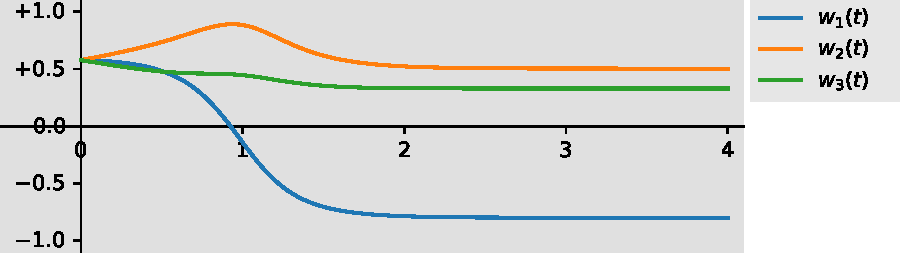
\includegraphics[width=\textwidth]{OjaFlow.pdf} 
\end{center}
\textbf{NOTE:} This result was obtained using $\vec{w}_0 = \frac{1}{\sqrt{3}} \vec{1}$. When you enter your result below, please use some random vector $\vec{w}_0$ with $\lVert \vec{w}_0 \rVert = 1$.
%%%%%
%%%%%
%%%%% enter your plot here, i.e. replace "placeholder.pdf" by the names of the graphics file you created
%%%%%
%%%%%
\begin{center}
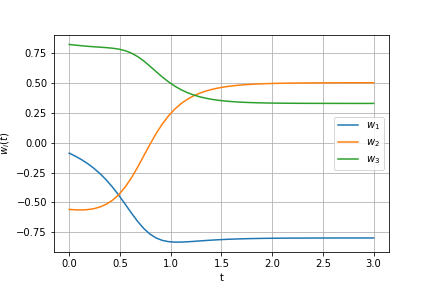
\includegraphics[width=0.7\textwidth]{Ex_02/Figures/OjaFlow.png} 
\end{center}
%%%%%
%%%%%
%%%%%
%%%%%
%%%%%

Compare the stable point the flow converges to to the leading eigenvector $\vec{u}_1$ you computed above. What do you observe? Also, experiment with different initial conditions / starting point for the flow. What do you observe?
\color{blue} \\[1ex]
%%%%%
%%%%%
%%%%% enter your discussion here
%%%%%
%%%%%
The two code fragments output the following:

$u_1$: [ 0.7988784 , -0.50319912, -0.32952077] \\
$w_t$: [ 0.79885363, -0.50324345, -0.32951316]

So one can see that $w_t$ is in fact an approximation of the leading eigenvector $u_1$ of the sample covariance matrix $C$. Depending on the initial condition for the flow it might happen that the the two vectors are of different sign, i.e. $w_t \approx -u_1$. This is represented by the cosine similarity converging to -1 instead of +1. However $-u_1$ is still a leading eigenvector of $C$.

\begin{figure}[h]
    \centering
    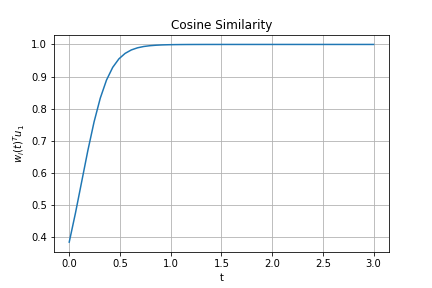
\includegraphics[width=0.45\textwidth]{Ex_02/Figures/CosSimilarity_positive.png}
    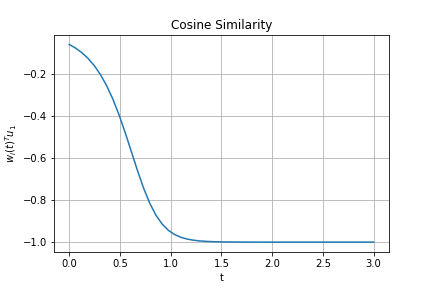
\includegraphics[width=0.45\textwidth]{Ex_02/Figures/CosSimilarity_negative.png}
    \caption{Cosine similaritity between $w(t)$ and $u_1$ for two different setups. Note that the two setups differ in the initial condition $w_0$, i.e. once $w_0^Tu_1 > 0$ (left) and once $w_0^Tu_1 < 0$ (right).}
    \label{fig:cos_sim}
\end{figure}

To get a bit more precise one can observe that the cosine similarity between the iterative approximations $w_i$ and the target $u_1$ never cross the x-axes (see figure \ref{fig:cos_sim}). What does this mean? Consider the plane containing the origin and for which $u_1$ is a normal vector. Then all the iterative approximations $w_t$ will be on the same side of the plane. This includes not just the randomly chosen initial condition $w_0$ but also the vector of convergence. Thus we see the following condition:

$$ w_t \approx sgn(w_0^Tu_1)u_1 $$

%%%%%
%%%%%
%%%%%
%%%%%
%%%%%
\color{black}






\subsection*{task 2.5 [5 points] \\[1ex] the Oja flow is isometric}

Prove the following claim: If the Oja flow 
\begin{equation}
\label{eq:flow2}
\dot{\vec{w}} = \bigl( \mat{I} - \vec{w} \trn{\vec{w}} \bigr) \mat{C} \vec{w}
\end{equation} 
starts with a unit vector $\vec{w}(0) = \vec{w}_0$ such that $\lVert \vec{w}_0 \rVert^2 = \trn{\vec{w}_0}{\vec{w}_0} = 1$, then it holds that
\begin{equation*}
\frac{d}{dt} \lVert \vec{w}(t) \rVert^2 = 0.
\end{equation*}

Observe that this is to say that, for unit vectors, the flow in \eqref{eq:flow2} is \emph{norm preserving} or \emph{isometric}.
\color{blue} \\[1ex]
%%%%%
%%%%%
%%%%% enter your discussion here
%%%%%
%%%%%
enter your proof here 
\begin{align*}
\frac{d}{dt} \lVert \vec{w} \rVert^2
& = \ldots
\end{align*}
%%%%%
%%%%%
%%%%%
%%%%%
%%%%%
\color{black}






\subsection*{task 2.6 [10 points] \\[1ex] the QR algorithm can sort!}

In task 1.3, you already implemented the QR algorithm and used it to compute the eigenvalues of a sample covariance matrix. Yet, amazingly (?), the QR algorithm can do much more \ldots

To see an example, implement the following procedure in Numpy / Scipy


\begin{enumerate}
\item Assume you were given a vector
\begin{equation*}
\vec{x} = \trn{[x_1, x_2, x_3, \ldots, x_n]}
\end{equation*}
consisting of $n$ elements $x_i \in \mathbb{R}$
\begin{python}
# get the dimension of the input vector
n = x.shape[0]
\end{python}

\item Create an $n \times n$ tri-diagonal matrix $\mat{X}$ whose main diagonal contains the elements of $\vec{x}$ and whose off diagonals contain a fixed small number $\epsilon$. In other words, create a matrix like this
\begin{equation*}
\mat{X} = 
\begin{bmatrix}
     x_1 & \epsilon \\
\epsilon &      x_2 & \epsilon \\
         & \epsilon &      x_3 & \epsilon \\
         &          &          &   \ddots & \epsilon \\ 
         &          &          & \epsilon &      x_n
\end{bmatrix}
\end{equation*}
\begin{python}
# build the tri-diagonal matrix with the vector x on the main
# diagonal and eps on both off-diagonals
off_diag = [eps] * (n-1)
X = np.diag(x) + np.diag(off_diag, k=1) + np.diag(off_diag, k=-1)
\end{python}

\item compute 
\begin{equation*}
\mat{X}' = \exp \bigl( \mat{X} \bigr)
\end{equation*}
\begin{python}
# compute the matrix exponential
X_prime = la.expm(X)
\end{python}

\item feed $\mat{X}'$ into the QR algorithm to obtain a matrix
\begin{equation*}
\mat{Y}' = \operatorname*{qrAlgorithm} \bigl( \mat{X}' \bigr)
\end{equation*}
\begin{python}
# apply the qr-algorithm
Y_prime = qr_alg(X_prime, **kwargs)
\end{python}

\item compute 
\begin{equation*}
\mat{Y} = \log \bigl( \mat{Y}' \bigr)
\end{equation*}
\begin{python}
# compute the matrix logarithm
Y = la.logm(Y_prime)
\end{python}
\end{enumerate}

\textbf{NOTE:} In this task, we write $\exp(\cdot)$ and $\log(\cdot)$ to denote the matrix exponential- and logarithm functions. Scipy provides them as \keyword{la.expm} and \keyword{la.logm}.

In order to work with a specific example, run you code with the following input and parameter
\begin{align*}
\vec{x}  & = \trn{[ 4, -3, 2, 7, 12, 1 ]} \\
\epsilon & = 0.0001
\end{align*}

Run your code four times using $t_{\text{max}} \in \{ 1, 5, 10, 50 \}$ iterations for the QR algorithm in step 4. After each run, print the diagonal entries of the matrix $\mat{Y}$ you obtain in step 5. What do you observe ?

\color{blue} \\[1ex]
%%%%%
%%%%%
%%%%% enter your discussion here
%%%%%
%%%%%

Just for completeness we insert the full code here:

\color{black}
\begin{python}
def qr_alg(A:np.ndarray, k:int =10) -> np.ndarray:
    # iterate for k iterations
    for _ in range(k):
        # decompose and build next matrix
        Q, R = la.qr(A)
        A = R @ Q
    # return last
    return A
def qr_sort(x:np.ndarray, eps:float =1e-4, **kwargs) -> np.ndarray:
    # get the dimension of the input vector
    n = x.shape[0]
    # build the tri-diagonal matrix with the vector x on the main
    # diagonal and eps on both off-diagonals
    off_diag = [eps] * (n-1)
    X = np.diag(x) + np.diag(off_diag, k=1) + np.diag(off_diag, k=-1)
    # compute the matrix exponential
    X_prime = la.expm(X)
    # apply the qr-algorithm
    Y_prime = qr_alg(X_prime, **kwargs)
    # compute the matrix logarithm
    Y = la.logm(Y_prime)
    # return the diagonal entries
    return np.diag(Y)
# create some sample input
x = np.asarray([4, -3, 2, 7, 12, 1], dtype=np.float32)
# apply for different iterations of the qr algorithm
for k in [1, 5, 10, 50]:
    sorted_x = qr_sort(x, k=k)
    sorted_x = np.rint(sorted_x)
    print("k=%i:\t" % k, sorted_x)
\end{python}
\color{blue}

The output looks as follows:

$k=k:  [ 4, -3,  2,  7, 12,  1]$ \\
$k=5:  [ 4, 12,  7,  2, -3,  1]$ \\
$k=10: [12,  4,  7,  2, -3,  1]$ \\
$k=50: [12,  7,  4,  2,  1, -3]$

One can observe that with increasing number of iterations of the QR algorithm, the output is being sorted better and better.

%%%%%
%%%%%
%%%%%
%%%%%
%%%%%
\color{black}




\end{document}
